\documentclass[article]{proc}
\usepackage{abstract}
\renewcommand{\abstractname}{}    % clear the title
\renewcommand{\absnamepos}{empty} % originally center

\titleConf{DAII\\
December 13th, 2019}
\city{Austin, TX, USA}
\usepackage{color}
\usepackage{graphicx}
\begin{document}
%%%%%%%%%%%%%%%%%%%%%%%%%%%%%%%%%%%%%%%%%%%%%%%%%%%%%%%%%%%%%%%%%%%%%%%%%%%%%%%%%%%%%%%%%%%%%%%%
\title{A quantitative framework for fire department unit purchasing decisions}
%For at least  authors with different addresses, use instead the following commands
\corrauthor[1]{Tyler C. Buffington}
\corremail{tyler.c.buffington@utexas.edu}
% \doi{http://dx.doi.org/10.1615/TFESC.XXX.XXX}
\address[1]{The University of Texas at Austin, Austin, TX, 78712, USA}

\maketitle
%%%%%%%%%%%%%%%%%%%%%%%%%%%%%%%%%%%%%%%%%%%%%%%%%%%%%%%%%%%%%%%%%%%%%%%%%%%%%%%%%%%%%%%%%%%%%%%%



\section{Introduction}



\section{Decision Overview}



\begin{table}[h]
\centering
\caption{An example of the resulting dataframe from the data processing described in this section. The first three minutes of May 14th are shown with minute 0 representing 12:00 AM, minute 1 representing 12:01 AM, etc. In this example, a call was placed at 12:01 AM, but not at the other minutes shown.}
\begin{tabular}{|l|l|l|l|}
\hline
\textbf{Date} & \textbf{Minute} & \textbf{Day of Week} & \textbf{Call placed?} \\ \hline
05/14/2019    & 0               & Tuesday              & 0                     \\ \hline
05/14/2019    & 1               & Tuesday              & 1                     \\ \hline
05/14/2019    & 2               & Tuesday              & 0                     \\ \hline
\end{tabular}
\label{minutedf}
\end{table}



\begin{figure}[!htb]
  \centering
  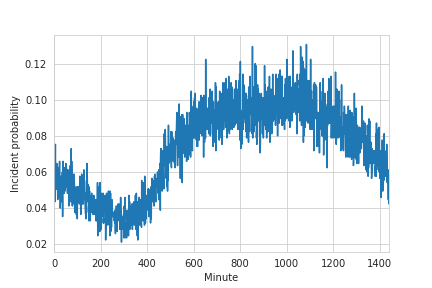
\includegraphics[width=12cm,keepaspectratio]{Figures/raw_signal.png}
  \caption{The aggregated probability of an emergency call for each of the 1,440 minutes of the day}
  \label{fig:raw_signal}
\end{figure}



\section{Modeling methodology}
\subsection{Data processing}
The starting point for the modeling effort described in this report is a large dataframe of incident data containing information on over 82,000 unit dispatches that occurred between May of 2015 and November of 2019. Each row of this dataframe is a dispatch of either an ALS or a suppression unit. The columns of the dataframe correspond to the unit id, the unit type, the time the unit was dispatched, the time the unit was cleared from the incident, where the incident occurred, and the station that houses the unit. Based on the location of the incident, each row also contains a \textit{first due} station entry. This entry is based on the fact that the department's jurisdictional region is divided into six smaller non-overlapping regions (one for each station) that each comprise the set of locations that are assigned to a station. Loosely speaking, the first due assignments are based on distance, meaning that for example, Station A's first due area is the set of locations that are closer to Station A than any other station. However, other factors affect these assignments and the boundaries of the first due areas are considered a ``take as given" for the purposes of this project.


The first step was to split the dataframe into two separate dataframes- one containing only ALS units and one containing only fire suppression units. Then each dataframe was grouped by the first due station corresponding to the location of the incident. For each station and each unit type, two response time arrays were generated- one corresponding to units that belong to the first due station, and one corresponding to units that came from other stations. These 



The author then built an algorithm that iterated through each dataframe and determined the units of the same type that were active at the moment each unit was dispatched; active means that a unit is between its dispatched timestamp and its cleared timestamp.
As a simple example, one can imagine three hypothetical unit dispatches- Unit A, which is dispatched at 12:00 PM and cleared at 1:00 PM, Unit B, which is dispatched at 12:30 PM and cleared at 1:30 PM, and Unit C, which is dispatched at 12:45 PM and cleared at 2:00 PM. Assuming these three dispatched comprise the entire dataset, then for Unit A, the algorithm would determine that no units were active at the time Unit A was dispatched. For Unit B, it would identify that Unit A was active at the time of dispatch, and for Unit C, it would identify that both Unit A and Unit B were active at the time of dispatch. 







\subsection{Distribution fitting}
For this project, several different methods of estimating hypothetical response time distributions were considered. Ideally, these methods should possess three attributes. First of all, they should be accurate, meaning that they produce estimations of the response time distributions that align with reality. Next, they should be modular, meaning that they can be easily recalculated for different modeling inputs. Finally, they should be computationally inexpensive so that an optimization routine can run many iterations in a relatively short amount of time. 


\subsection{Optimization}





\begin{equation}
p(x) = A_0 + \sum_{n=1}^{N} A_ncos(nw_0x) + B_nsin(nw_0x)
\label{eq:fourier_poly}
\end{equation}

\subsection{Value quantification}




\section{Insights and recommendations}


\section{Conclusions and future work}




\bibliographystyle{Bibliography_Style}
\scriptsize{
\bibliography{./References}
}

\end{document}
